\chapter{Linear Programming}\label{chap:lp}
    \section{Linear Programming Problems}
        A linear programming (LP) problem is an \textit{optimization} problem in the form
        \begin{equation}\label{eq:lp_problem}
            \begin{cases}
                \text{min } f(\underline{x})\\
                \text{s.t. } \underline{x} \in X \subseteq \mathbb{R}^n
            \end{cases}
        \end{equation}
        where:
        \begin{itemize}
            \item $f: X \,\rightarrow\, \mathbb{R}$ is a \textit{linear function}
            \item the \textit{feasible region} $X \subseteq \mathbb{R}^n$ is a combination of linear functions.
        \end{itemize}
        \begin{definition}
            $\underline{x}^* \in \mathbb{R}^n$ is an \emph{optimal solution} of the LP \eqref{eq:lp_problem} if $f(\underline{x}^*) \leq f(\underline{x}), \forall \underline{x} \in X$
        \end{definition}
        LP problems can also be formulated with matrixes:
        \begin{equation}
            \begin{cases}
                \text{min } z = \underline{c}^t\, \underline{x}\\
                A\underline{x} \geq \underline{b}\\
                \underline{x} \geq \underline{0}
            \end{cases}
        \end{equation}

        \paragraph{Assumptions of LP Models}
            LP models and the algorithms operating on them work under several assumptions:
            \begin{enumerate}
                \item \underline{Linearity} of the objective function and constraints
                \item \underline{Divisibility}: The variables can take fractional (rational) values.
                \item \underline{Parameters} are considered as constants which can be estimated with a sufficient degree of accuracy.
            \end{enumerate}
        \textbf{Note}: LP "sensitivity analysis" allows to evaluate how sensitive an optimal solution is
        with respect to small changes in the parameter values (see end of Chapter \ref{chap:lp}).
    \section{LP Problems Forms}
        The most general for for a linear programming model we can define is:
        \begin{equation}
            \begin{cases}
                \text{min/max } z = \underline{c}^t\, \underline{x}\\
                A_1\underline{x} \geq \underline{b_1}\\
                A_2\underline{x} \leq \underline{b_2}\\
                A_3\underline{x} = \underline{b_3}\\
                x_j \geq 0 &\text{for some \emph{j}}\\
                x_j \text{ free} & \text{for others j}
            \end{cases}
        \end{equation}
        This form is usually referred to as \textit{canonical form}.

        \paragraph{Standard Form}
            The standard form is the "most restrictive" one, and also one of the easiest to work with
            \begin{definition}[Standard form]
                \begin{equation}
                    \begin{cases}
                        \text{min } z = \underline{c}^t\, \underline{x}\\
                        A\underline{x} = \underline{b} & \text{only \emph{equality constraints}}\\
                        \underline{x} \geq \underline{0} & \text{all \emph{nonnegative} variables}
                    \end{cases}
                \end{equation}
            \end{definition}
            In this form, all constraints must be equalities, and all variables must be non negative.\\
            \textbf{Pay attention}: in the original general model, we have the non-negativity constraints only on \underline{some} variables.

            \subparagraph{Transforming to Standard Form}
                We can easily transform a general formulation of a LP problem in standard one by applying these simple transformations:
                \begin{itemize}
                    \item $\max(\underline{c}^t\underline{x}) = -\min(-\underline{c}^t\underline{x})$ to change objective function
                    \item all inequalities are transformed adding a \emph{slack} variable:
                        \begin{equation}
                            \underline{a}^t\underline{x} \leq \underline{b} \Rightarrow
                                \begin{cases}
                                    \underline{a}^t\underline{x} + s = \underline{b}\\
                                    s \geq 0
                                \end{cases}
                        \end{equation}
                        or a \emph{surplus} variable in case it's a $\geq$ inequality
                        \begin{equation}
                            \underline{a}^t\underline{x} \geq \underline{b} \Rightarrow
                                \begin{cases}
                                    \underline{a}^t\underline{x} - s = \underline{b}\\
                                    s \geq 0
                                \end{cases}
                        \end{equation}
                    \item when a variable is unrestricted in sign it's "splitted" in its positive and negative part:
                        \begin{equation}
                            x_j \in \mathbb{R} \Rightarrow
                                \begin{cases}
                                        x_j = x_j'-x_j''\\
                                        x_j' \geq 0\\
                                        x_j'' \geq 0
                                \end{cases}
                        \end{equation}
                \end{itemize}

    \section{Geometry of a LP Problem}
        \subsection{Feasible Region as an Hyperplane}
            \begin{definition}[Level curve]
                A level curve of value $z$ of a function $f$ is the set of points in $\mathbb{R}^n$ where $f$ is constant and takes value $z$.
            \end{definition}
            
            \begin{definition}
                \begin{itemize}
                    \item[]
                    \item[] $ H = \{x \in \mathbb{R}^n \,\vert\, \underline{a}^tx = \underline{b}\}$ is an \emph{hyperplane};
                    \item[] $H^- = \{x \in \mathbb{R}^n \,\vert\, \underline{a}^tx \leq \underline{b}\}$ is an \emph{affine half-space}.
                \end{itemize}
           \end{definition}
           \textbf{Note}: Each inequality constraint ($a^Tx \leq b$) defines an affine half-space in the variable space.\\

            So, the \textit{feasible region} of an LP problem, defined as \textit{a region delimited by hyperplanes}, is called a \textit{polyhedron}. A polyhedron (so a polygon in two dimension, a 3D figure in three dimension and so on) is a \underline{convex} set of $\mathbb{R}$ as generated by convex sets.
            \begin{figure}[H]
                \centering
                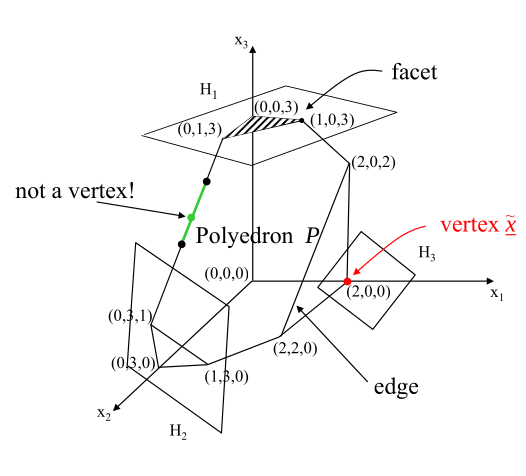
\includegraphics{./images/Polyhedron1.png}
            \end{figure}
            \begin{definition}[Convex combination]
                We call a convex combination a linear combination where all coefficients are non negative and sum to 1.
            \end{definition}
            \begin{definition}[Vertex]
                A \emph{vertex} of $P$ is a point of $P$ which cannot be expressed as a convex combination of two other distinct points of $P$.    
            \end{definition}
            Don't worry if you're confused: all "polyhedra theory" has a lot of dark spots\footnote{check out they wikipedia page}.
            \begin{property}
                A non-empty polyhedron $P = \{\underline{x} \in \mathbb{R}^n : A\underline{x} = b, x \geq 0\}$ (in standard form) or
                $P = \{\underline{x} \in R^n : A\underline{x} \geq b, x \geq 0\}$ (in canonical form) has a finite number ($\geq$ 1) of vertices.
            \end {property}
            \textbf{Example}: a polyhedron with only one vertex is a quarter of plane, for example.\\

           
            \begin{theorem}[Representation of polyhedra - Weyl-Minkowski]
                Every point $x$ of a polyhedron $P$ can be expressed as a convex combination of its vertices $x^1 , . . . , x^k$ plus (if needed) an unbounded feasible direction $d$ of $P$:
                $$ \underline{x} = \lambda_1 \underline{x}^1 + ... + \lambda_k \underline{x}^k + d$$
                where the multipliers $\lambda_i \geq 0$ satisfy $\lambda_1 + ... + \lambda_k = 1$.
            \end{theorem}
            So, we can represent \textit{every point of a polyhedron} as a convex combination of its \textit{vertices} plus (if needed) a vector that never ends inside the polyhedron (for unbounded polyhedron).

            \begin{figure}[H]
                \centering
                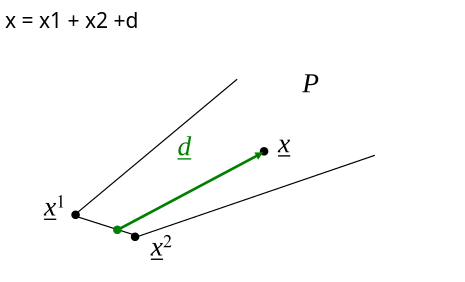
\includegraphics{./images/Polyhedron2.png}
                \caption{Every point of this unbounded polyhedron can be represented as a combination of $x_1$ and $x_2$ and $\underline{d}$, where $\underline{d}$ is called \textit{unbounded feasible direction} of the polyhedron.} 
            \end{figure}
            Only for completeness, we can define bounded polyhedron as:
            \begin{definition}[Polytope]
                A polytope is a bounded polyhedron, that is, it has the only unbounded feasible direction $d = 0$.
            \end{definition}
            \subsection{Fundamental Theorem of Linear Programming}
                \begin{theorem}[Fundamental theorem of Linear Programming]
                Consider a LP $min\{c^T x : x \in P\}$, where $P \subseteq R^n$ is a non-empty polyhedron of the feasible solutions (in standard or canonical form).\\
                Then either:
                \begin{itemize}
                    \item  there exists (at least) one optimal vertex or
                    \item the value of the objective function is unbounded below on $P$.
                \end{itemize}
               
                \end{theorem}
                This foggy theorem has a simple intuitive interpretation, in my mind: the feasible region is represent as a subset of $\mathbb{R}$ and reprents \textit{all the solutions of the system of constraints}. To minimize the objective function, we must "move around" this subspace in a well-defined direction, that is the opposite of the gradient of the objective function itself. Being this a \textit{straight line}, we will eventually hit a boundary of the polyhedron. We could then "slide" onto it until we are "stuck" and every move we make is not anymore bettering the solution. This can happen \textit{only} on the intersection of boundaries (so the vertices), because it's the only point where a "direction" to better the solution finds his boundary\footnote{I find this mumbo jumbo more clear than the slides definition, ok? In my head it's clear this way.}.\\
                
                This theorem allows us to do determine a priori which are our solutions, just looking at the way the feasible region is defined. Also, being \textit{finite}, we can cycle through the solutions to "easily" find the right one.

    \section{Algebraic Characterization of the LP Problem}
        We've seen we can exploit the geometry of the feasible region to find the solutions. We need an algebraic formulation to do that algorithmically.

        \subsubsection{The Feasible Vector Space}
            Classic LP problem: $P=\{x \in \mathbb{R} \,\vert\, Ax = b, x \geq \underline{0}\}$ in standard form. We assume from now on that $A$ is full rank. This leads to two possible scenarios:
            \begin{itemize}
                \item $A$ is a square matrix $\Rightarrow$ there exists only a \textit{unique} solution to the system: $x = A^{-1}b$.
                \item $A$ is a rectangular matrix with more columns than rows: this leads to infinite solutions of the system.
            \end{itemize}
            Obviously, having the exact number of constraints equal to the variables one is not common. We focus on the second case.\\
            If we partition the matrix $A = [B \,\vert\, N]$, where $B$ is a basis\footnote{set of linearly indipendent vectors} and $N$ the "remaining" vectors, we can redefine the solutions' vector as:
            \begin{equation}
                x = (x_B,\, x_N)
            \end{equation}
            where the two components of the vector will be long as the rank of the matrix and the lenght of the remaining matrix. We then substitute into the feasible region definition
            \begin{equation}
                Bx_{B} + Nx_{N} = \underline{b}
            \end{equation}
            and so
            \begin{equation}
                x_{B} = B^{-1}\underline{b} - B^{-1}Nx_{N}
            \end{equation}
            from this last equation, we can define
            \begin{itemize}
                \item a \underline{basic solution} is a solution setting all non base variables $x_{N}$ to zero, so $x_B = B^{-1}\underline{b}$
                \item a \underline{basic \textit{feasible} solution} is a basic solution that has all components greater or equal to zero
                \item the variable in $x_B$ are called \underline{basic variables} and the ones in $x_N$ \underline{non basic variables}
            \end{itemize}
            Now we link the algebraic formulation with the geometrical interpretation:
            
            \begin{theorem}
                $x \in \mathbb{R}^n$ is a \textit{basic feasible solution} $\Leftrightarrow$ $x$ is a \textit{vertex} of $P = \{x \in \mathbb{R}^n \,\vert\, Ax = \underline{b}, x \geq \underline{0}\}$
            \end{theorem}

    \section{The Simplex Method}
        Dantzig's simplex method is an algorithm to find the best basic feasible solution of a LP problem:
        it examines a sequence of BFSs\footnote{Basic feasible solutions} with \textit{non increasing objective function values} until an optimal solution is reached, or the problem is found to be \textit{unbounded}.

        \subsubsection{The Algorithm}
            \begin{enumerate}
                \item check for infeasibility of the problem
                \item find an initial vertex
                \item move from a current vertex to a \textit{better adjacent vertex} (or establish that the problem is unbounded)
                \item determine if the current vertex is \textit{optimal}
            \end{enumerate}

            \paragraph{Infeasibility Check}
            To check if a problem is infeasible, we create an auxiliary problem with artificial variables (from the original problem) as:
                \begin{equation}
                    P = 
                    \begin{cases}
                        \min z = \underline{c}^t x\\
                        Ax = \underline{b}
                        x \geq \underline{0}
                    \end{cases}
                \end{equation}
                \begin{equation}
                    P_{aux} = 
                    \begin{cases}
                        \min v = \sum_{i = 1}^m y_i\\
                        Ax + Iy= \underline{b}\\
                        x \geq \underline{0}, y \geq \underline{0}
                    \end{cases}
                \end{equation}
                obviously, there exists a BFS composed by all elements in \emph{y}. We face two cases now:
                \begin{enumerate}
                    \item $v > 0$ the problem is \textit{\textbf{infeasible}}
                    \item if $v = 0$, the problem is feasible and we must manipulate the matrix in order to obtain a BFS that only depends on the original $x_i$ variables
                \end{enumerate}
                Don't forget we have to turn to the original problem and recompute the objective function.

            \paragraph{Initial Vertex Selection}
                The selection of a starting initial BFS is a problem per se. If the problem is easy enough we'll have the initial matrix already in a $A = [N \,\vert\, I]$ form, where \emph{I} represents the identity matrix $\Rightarrow$ a basic feasible solution. In that case, we have already a perfect indication of which variables are in the basis and at which cost, so we can directly go to the "movement" phase (that's the one that really optimizes the objective function value).\\
                In the other case (that's obviously more realistic) we have to resort again at the "auxiliary problem" with artificial variables: the initial basis we find is the one determined by the $y_i$ vectors.

            \paragraph{Movement Across Vertices}
                To "move" from a vertex to another means to swap some of the basic vertices out of the solution and "bring in" some of the vectors that were in the $N$ matrix. \textit{Algebrically}, this means to \textit{expressing the basic variables in terms of the non basic ones}. \textbf{Remember}: non basic variables are set to \textbf{zero}. Algorithmically, this is done through a simple pivoting operation on the combined $[B\vert N]b$ matrix.\\
                Given $Ax = \underline{b}$
                \begin{enumerate}
                    \item select a coefficient $a_{rs} \neq 0$ of table $A$ where \emph{r} is the row index and \emph{s} is the column index
                    \item divide row \emph{r} for $a_{rs}$ (also in order to have $a_{rs} = 1$)
                    \item for alla other rows, subtract row \emph{r} multiplied by the coefficient on column \emph{s}: that is, $a_{is}$
                \end{enumerate}
                This will render the \emph{s} column all zeroes except the 1 on row \emph{r}. Don't forget we're applying this procedure also the the $\underline{b}$ vector.
                \begin{figure}[H]
                    \centering
                    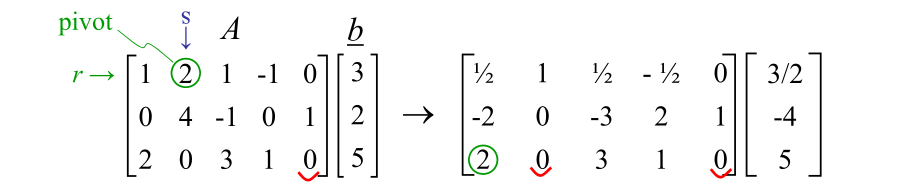
\includegraphics[width = \textwidth]{./images/Simplex1.png}
                \end{figure}
                The choice of \emph{r} and \emph{s} are crucial: in fact, they select which variable enters the basis (through the pivot column) and which leaves it (through the pivot row). This choice can be taken
                \begin{itemize}
                    \item randomly
                    \item using heuristics
                    \item usign \textbf{Bland's rule}, that also avoid cycles in the algorithm
                \end{itemize}

                \subparagraph{Bland's Rule}
                    Bland's rule dictate a choice for rows and columns to enter/leave the basis. It states:
                    \begin{enumerate}
                        \item select \emph{s} the \textit{first column with negative reduced cost}
                        \item then select \emph{r} the row with the \textit{smallest} $\frac{b_r}{a_{rs}}$ ratio \textbf{among the positive ones}
                    \end{enumerate}
                    This simple criterion avoids cycles in the Simplex algorithm, that can be stuck in a vertex for some degenerate LP problems. In practice, due to the additional complexity added and the rarity of such problems, Bland's rule is never used.

                \subparagraph{Tableau Representation}
                    As spoiled when talking about movement across
                    vertices, the Simplex method has a peculiar
                    way to represent the matrixes
                    and vectors it uses to ease the computing problem.\\
                    Given
                    \begin{equation}
                        P = 
                        \begin{cases}
                            z=\underline{c}^t x\\
                            Ax = \underline{b}
                        \end{cases}
                    \end{equation}
                    We initialize the tableau of values as
                    \begin{figure}[H]
                        \centering
                        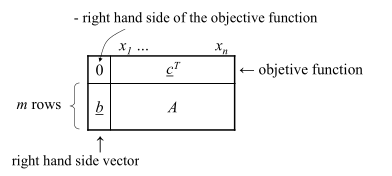
\includegraphics[width = \textwidth]{./images/Simplex2.png}
                    \end{figure}
                    Then we proceed (through the pivoting operation) to put the tableau in canonical form:
                    \begin{figure}[H]
                        \centering
                        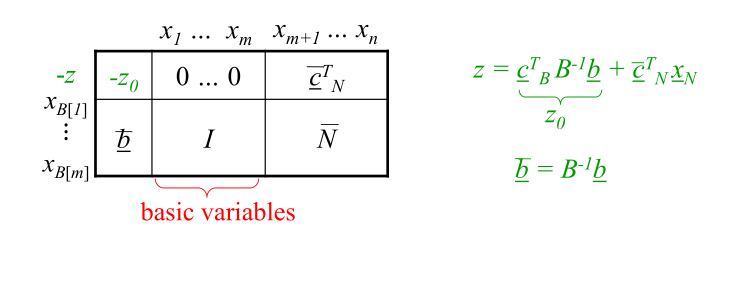
\includegraphics[width = \textwidth]{./images/Simplex3.png}
                    \end{figure}


            \paragraph{Optimality Check}
                To check if a solution is optimal we cannot only watch the feasible region, we must take into account also the objective function. We repeat the reasoning made for finding the expressions of BFSs: given $x_B = B^{-1}\underline{b} - B^{-1}N\underline{x_N}$ basic solution and posing $x_N$ equal to zero to find the basic feasible solution, we can express the $\{\min(\underline{c}^tx)\}$ objective function as
                \begin{equation}
                    \underline{c}^tx = (c_B, c_N) * \begin{pmatrix} x_B \\ x_N \end{pmatrix} = 
                        \begin{pmatrix}
                            B^{-1}\underline{b} - B^{-1}N\underline{x_N} \\
                            x_N
                        \end{pmatrix}
                \end{equation}
                we can now separate
                \begin{equation}
                    \underline{c}^tx = \underbrace{c_B^tB^{-1}b}_{z_0} + \underbrace{(c_N^t - c_B^tB^{-1}N)x_N}_{\underline{\overline{c_N}}}
                \end{equation}
                where
                \begin{itemize}
                    \item $z_0$ is a \textit{constant value} and is called cost of the basic feasible solution
                    \item the second term $\underline{\overline{c_N}}$ is a function \textit{only of the non basic variables} and is the \textit{reduced cost} o the non basic variables
                \end{itemize}
                We can also define de vector of reduced costs wrt the basis itself: $\underline{\overline{c}} = \underline{c}^t -\underline{c}_B^tB^{-1}A$ that is
                \begin{equation}
                    \begin{pmatrix}
                        c_B^t - c_B^tB^{-1}B \\
                        c_N^t - c_B^tB^{-1}N
                    \end{pmatrix}
                    =
                    \begin{pmatrix}
                        0 \\
                        \underline{\overline{c_N}}
                    \end{pmatrix}
                \end{equation}
                The reduced costs gives a measure on how much the objective function changes wrt a change in the value of the variable. Also, they provide a sufficent (but not usually necessary) condition for \textbf{optimality}: if all reduced costs of non basic variables are non negative, then the basic feasible solution associated to that non negative variables is optimal. So, more formally:\\
                Given $P = \{\underline{c}^tx : [B \vert N]x = \underline{b}, x \geq \underline{0}\}$
                \begin{equation}
                    \underline{\overline{c_N}} \geq \underline{0} \Rightarrow (x_B, x_N) \text{ s.t. } x_B = B^{-1}\underline{b} \geq \underline{0} \,\wedge\, x_N = \underline{0}, x_B \text{ is optimal}
                \end{equation}

    \section{Duality}
        The \textbf{duality} concept for linear programming can be explained as: to any minimization (maximization) LP problem we can associate a closely related maximization (minimization) LP problem \textit{based on the same parameters}. For example, the famous maximum network flow problem is the dual of the minimum capacity cut problem.

        \subsubsection{Building the Dual Problem}
            Given a maximization problem $P = \{\max \underline{c}^tx, Ax \leq \underline{b}\}$ any feasible solution provides a \textit{lower bound} of the objective function value. "Which one is the best lower bound"? Can we "flip" the problem to a minimization one?\\
            The basic idea is to find a \textit{linear combination of the constraints} in such a way that the obtained value for the constraints \textit{dominates}\footnote{has a higher value} the objective function. So, a new set of variables should be introduced (the coefficents of the linear combination) and should be linked to the \textit{coefficents of the objective value}. These new constraints will create the new feasible region. The objective function the must be changed also: it has to tune each new constraint with the original value of such equation. An example will do the trick.

            \paragraph{Example}
                Given
                \begin{equation}
                    \begin{cases}
                        \max z = 4x_1+x_2+5x_3+3x_4 \\
                        \begin{pmatrix}
                            1 & -1 & -1 & 3 \\
                            5 & 1 & 3 & 8 \\
                            -1 & 2 & 3 & -5
                        \end{pmatrix}
                        \times
                        \begin{pmatrix}x_1 \\ x_2 \\ x_3 \\ x_4\end{pmatrix}
                        \leq
                        \begin{pmatrix}1 \\ 55 \\ 3\end{pmatrix} \\
                        x \geq \underline{0} 
                    \end{cases}
                \end{equation}
                If we just multiply the second row of matrix \emph{A} for $\frac{5}{3}$, we obtain a disequality that dominates the objective function. We also obtain such a constraint if we add the second and the third row of the matrix. This two operations generate a \textit{valid constraint} that also \textit{brings information about the objective function}: it gives the obj an upper bound.\\
                Generalizing this reasoning, we can define a linear combination of the constraints, and also linarly combine them with the right hand side vector \emph{b}, to have actually a whole new set of constraints that is also consistent
                \begin{equation}
                    y_1 * (\text{ first line of A }) + y_2 * (\text{ second line of A }) + y_3 * (\text{ third line of A }) \leq y_1 + 55y_2 + 3y_3
                \end{equation}
                Now we can factorize the above equation in order to isolate the $x_i$ variables. Then, we turn back to imposing that the \textit{coefficient for $x_i$ must be greater or equal to the one of the objective function} in order to dominate it.
                \begin{equation}
                    \begin{pmatrix}
                        1 & 5 & -1 \\
                        -1 & 1 & 2 \\
                        -1 & 3 & 3 \\
                        3 & 8 & -5 \\
                    \end{pmatrix}
                    \times
                    \begin{pmatrix}y_1 \\ y_2 \\ y_3\end{pmatrix}
                    \geq
                    \begin{pmatrix} 4 \\ 1 \\ 5 \\ 3 \end{pmatrix}
                \end{equation}
                we can see as the last vector is just the $\underline{c}$ vector of the original problem. Given that we're now looking for an upper bound of \emph{z}, and also the \textit{lowest} upper bound, the dual problem will be a minimization problem; also, every "constraint coefficient" variable will contribute to the objective function proportionally to their right hand side coefficient of the original problem. We can now formulate the full dual problem:
                \begin{equation}
                    \begin{cases}
                        \min v = y_1 + 55 y_2 + 3 y_3 \\
                        \begin{pmatrix}
                            1 & 5 & -1 \\
                            -1 & 1 & 2 \\
                            -1 & 3 & 3 \\
                            3 & 8 & -5 \\
                        \end{pmatrix}
                        \times
                        \begin{pmatrix}y_1 \\ y_2 \\ y_3\end{pmatrix}
                        \geq
                        \begin{pmatrix} 4 \\ 1 \\ 5 \\ 3 \end{pmatrix} \\
                        y \geq \underline{0}
                    \end{cases}
                \end{equation}

        \subsubsection{General Form of the Dual Problem}
            As could be derived from the example, the relation between th \textbf{primal} and \textbf{dual} problem is
            \begin{equation}
                (P) = 
                \begin{cases}
                    \max z = \underline{c}^tx \\
                    Ax \leq \underline{b} \\
                    x \geq \underline{0}
                \end{cases}
            \end{equation}
            \begin{equation}
                (D) = 
                \begin{cases}
                    \min v = \underline{b}^ty \\
                    A^ty \geq \underline{c} \\
                    y \geq \underline{0}
                \end{cases}
            \end{equation}
            The duality relation is symmetric: if \emph{D} is the dual of \emph{P}, then the dual of \emph{D} is \emph{P}.\\
            When dealing with problems in standard form, the non negativity constraint on the vector $y$ is not more needed.\\
            Another formulation for this problem that keeps into account the basic and nonbasic solutions is:
            \begin{multicols}{2}
                \begin{equation}
                    (P) = 
                    \begin{cases}
                        \min z = c_Bx_B + c_Nx_N \\
                        Bx_b + Nx_N = b \\
                        x_B,\, x_N \geq \underline{0}
                    \end{cases}
                \end{equation}
                \break
                \begin{equation}
                    (D) = 
                    \begin{cases}
                        \max v = yb \\
                        yB \leq c_B \\
                        yN \leq c_N
                    \end{cases}
                \end{equation}
            \end{multicols}

        \subsubsection{Weak Duality Theorem}
            Given the classical formulation for a linear programming problem and its dual:
            \begin{multicols}{2}
                \begin{equation}
                    (P) = 
                    \begin{cases}
                        \max z = \underline{c}^tx \\
                        Ax \leq \underline{b} \\
                        x \geq \underline{0}
                    \end{cases}
                \end{equation}
                \break
                \begin{equation}
                    (D) = 
                    \begin{cases}
                        \min v = \underline{b}^ty \\
                        A^ty \geq \underline{c} \\
                        y \geq \underline{0}
                    \end{cases}
                \end{equation}
            \end{multicols}
            the \textit{weak duality theorem} states that for every feasible solution $\underline{\overline{x}} \in X$ of $(P)$ and every feasible solution $\underline{\overline{y}} \in Y$ of $(D)$ we have
            \begin{equation}
                \underline{b}^t\underline{\overline{y}} \leq \underline{c}^t\underline{\overline{x}}
            \end{equation}
            This is easy to visualize if we imagine the two problems (and in particular, the two feasible regions) as opposite but with the same objective: one is trying to reach the optimal solution by increasing the objective function value, the other doing the opposite reducing it. This leads us to the next important property of dual problems:

        \subsubsection{Strong Duality Theorem}
            Given primal and dual problem as in (31) and (32), and given that they are both \textit{bounded} and \textit{feasible}, then if $x^*$ is an optimal solution for $(P)$ and $y^*$ is an optimal solution for $(D)$ we have that
            \begin{equation} \underline{c}^tx^* = \underline{b}^ty^* \end{equation}
            \begin{minipage}{0.5\linewidth}
                Again, this is just an extension of what we've said for the weak duality theorem: the visualization is also very simple, as shown in the figure
            \end{minipage}
            \begin{minipage}{0.5\linewidth}
                \begin{figure}[H]
                    \centering
                    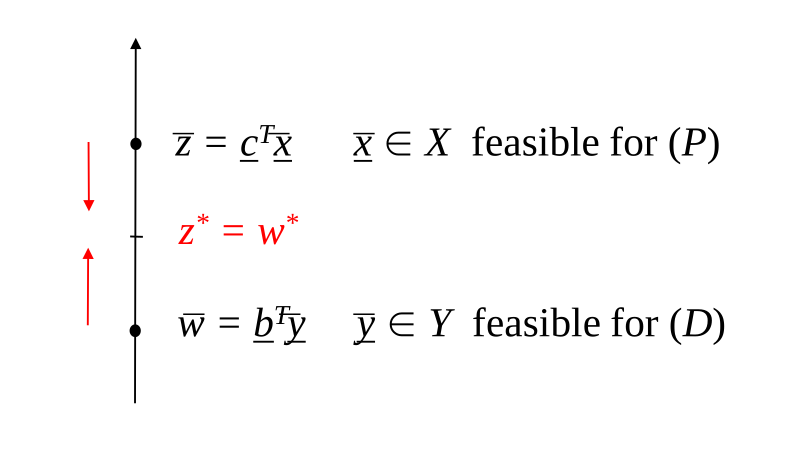
\includegraphics[width = \textwidth]{./images/Duality1.png}
                    \caption{Relation between feasible regions and optimal solutions of dual problems.}
                \end{figure}
            \end{minipage}
            \vspace{0.5cm}
            
            in the end, we have 4 possible cases out of 9 possible combination of problems, that are explained in the table below:
            \begin{center}
                \begin{tabular}{ m{2.5cm} || m{4cm} | m{4cm} | m{4cm} | }
                    & $\exists$ an optimal solution & unbounded problem & infeasible problem \\
                    \hline
                    \hline
                    $\exists$ an optimal solution & Granted by the strong duality theorem & Not possible (SDT) & Not possible (SDT) \\
                    \hline
                    unbounded problem &  & not possible (WDT) & consequnce of weak duality theorem \\
                    \hline
                    infeasible problem &  &  & only possible combination for empty feasible region\\
                    \hline
                \end{tabular}
            \end{center}
            where obviously columns and rows represent the possible condition of the primal and dual problem. As said, the relation is symmetric (so only half of the matrix is shown) and SDT and WDT means Strong Duality Theorem and Weak Duality Theorem.

        \subsubsection{Optimality Conditions}
            The strong duality theorem gives us a powerful tool to prove the optimality of a solution of the linear problem: if we find $x^*$ optimal solution for the primal problem and $y^*$ optimal solution for the dual, it must hold that $\underline{c}^tx^* = \underline{b}^ty^*$. This can be easily proven by substituting the definition of the vectors inside the equation given:
            \begin{equation}
                \begin{cases}
                    Ax^* = \underline{b} \\
                    A^ty^* = \underline{c} \\
                    \Rightarrow \,\, y^{*t} \underline{b} = y^{*t}Ax^* = \underline{c}^tx^*
                \end{cases}
            \end{equation}

        \subsubsection{Complementary Slackness}
        Following along the reasoning that gaves us the new Optimality Conditions, we can see a lso a relation between \textit{slack variables} of optimal solution. Let's say $x^* \in X \text{ and } y^* \in Y$ optimal solutions for the primal and the dual problem respectively. We can notice that
        \begin{equation}
            \begin{cases}
                \forall i \,\vert\, y_i^*(a_i^tx^*-\underline{b}_i) = 0 \\
                \forall j \,\vert\, (\underline{c}_i^t - y^{*t}a_j)x_j^* = 0
            \end{cases}
        \end{equation}
        Where \emph{i} and \emph{j} represents respectively the row index and the column index of the \emph{A} table. We can see that at \textit{optimality}, the product of each variable with the corresponding slack variable of the constraint of the relative dual is null. This \textit{again} gives us a way to easily detect optimality in a solution and to find the dual one: it's enough to check the complementary slackness equations once found a solution.

    \section{Sensitivity Analisys}
			"How much does an optimal solution change wrt the variations of some of its parameters?"\\
			This is sensitivity analysis, so calculate and quantify the effect produced on the optimal objective function value by a variation in the parameter value. This is useful when adjustments must be made, and we have to choose which parameter ensures the maximum or minimum variation overall. Remember: in sensitivity analysis \textit{everything} is a parameter, from the optimal solution values to the right hand side vector of the feasible region definition.

			\subsubsection{Optimality Intervals}
				A direct application of sensitivity analysis is to find the interval in which a basis \emph{B} remains optimal\footnote{so that $B^{-1}\underline{b}$ remains non negative with $x_N$ set to zero, and th reduced costs of the variables in the basis remain non negative too.}. In this case, we can vary the cost coefficents and the right hand side termns in order to verify the intervl of validity of a base.

				\paragraph{Tweaking the \emph{\underline{b}} Vector}
					We have the optimal solution $\underline{x}^* = \begin{pmatrix} B^{-1}(\underline{b}) \\ \underline{0} \end{pmatrix}$, we modify \emph{slightly} the solutions vector, we obtain:
					\begin{equation}
						x^* = 
						\begin{pmatrix}
							B^{-1} ( \underline{b}\, +\, \delta \underline{e} ) \\
							\underline{0}
						\end{pmatrix}
					\end{equation}
					where as usual the nullifiedpart of the vector is the one associated to the non basic variables, and \emph{e} represents a column of the identity matrix. In systesys, we're modifyin just a single entry of the solutions vector, by $\delta$. We just apply the definition of optimality for a basis and have that \textit{B remains optimal as long as}
					\begin{equation}
						B^{-1} ( \underline{b}\, +\, \delta \underline{e} ) \geq \underline{0} \,\Rightarrow\, B^{-1}\underline{b} \geq -\delta B^{-1} \underline{e}
					\end{equation}
					Obviously, changing the value of the basic vectors impacts the value of the objective function, which goes from $\{\underline{c}^tB^{-1}\underline{b}\}$ to $\{ \underline{c}^tB^{-1} ( \underline{b}\, +\, \delta \underline{e} ) \}$.

				\paragraph{Tweaking the \emph{\underline{c}} Vector}
					We increment just as before the cost coefficient vector as $\underline{c}' = \underline{c}\, +\, \delta \underline{e}$. The basis remains optimal as long as
					\begin{equation}
						\underline{c}_N^{'t}\, -\, \underline{c}_B^{'t}B^{-1}N \geq \underline{0}
					\end{equation}
					In this case, we're changing the objective function value, but \textit{differently from the previous case} the $x^*$ vector remain unchanged.
